\renewcommand*{\arraystretch}{1.1}

\subsection*{Interactive / update / 7}
\label{sec:interactive-update-07}

\noindent\begin{tabularx}{\queryCardWidth}{|>{\queryPropertyCell}c|X|}
	\hline
	query & Interactive / update / 7 \\ \hline
%
	title & Add Comment \\ \hline
%
    pattern & \hfill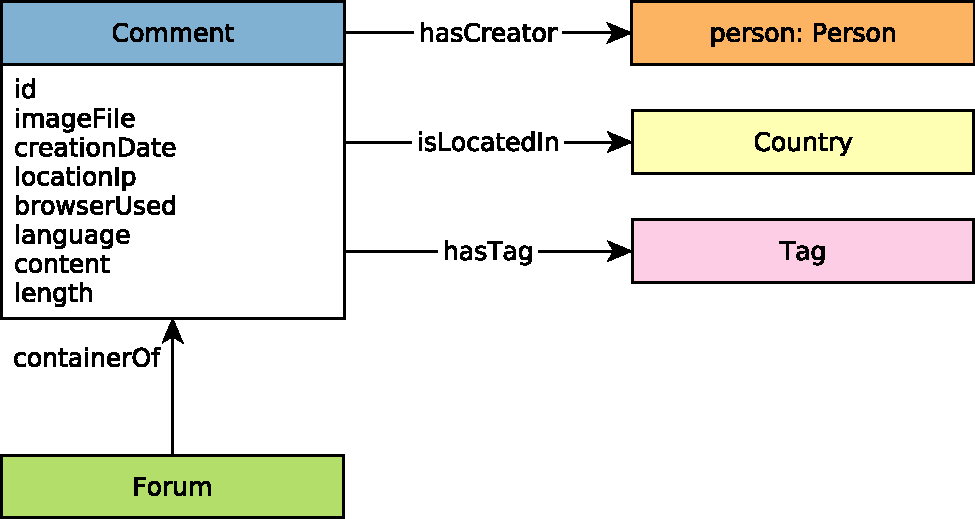
\includegraphics[scale=\patternscale,margin=0cm .2cm]{patterns/interactive-update-07}\hfill\vadjust{} \\ \hline
%
	desc. & Add a Comment replying to a Post/Comment to the social network.
 \\ \hline
%
	
%
    
        params &
        \innerCardVSpace{\begin{tabularx}{\attributeCardWidth}{|>{\paramNumberCell}c|>{\varNameCell}M|>{\typeCell}m{\typeWidth}|Y|} \hline
        \cellcolor{parameter} \color{white} \footnotesize $\mathsf{1}$ &Comment.id& ID &  \\ \hline
        \cellcolor{parameter} \color{white} \footnotesize $\mathsf{2}$ &Comment.creationDate& DateTime &  \\ \hline
        \cellcolor{parameter} \color{white} \footnotesize $\mathsf{3}$ &Comment.locationIp& String &  \\ \hline
        \cellcolor{parameter} \color{white} \footnotesize $\mathsf{4}$ &Comment.browserUsed& String &  \\ \hline
        \cellcolor{parameter} \color{white} \footnotesize $\mathsf{5}$ &Comment.content& Text &  \\ \hline
        \cellcolor{parameter} \color{white} \footnotesize $\mathsf{6}$ &Comment.length& 32-bit Integer &  \\ \hline
        \cellcolor{parameter} \color{white} \footnotesize $\mathsf{7}$ &Comment-hasCreator->Person.id& ID &  \\ \hline
        \cellcolor{parameter} \color{white} \footnotesize $\mathsf{8}$ &Comment-isLocatedIn->Country.id& ID &  \\ \hline
        \cellcolor{parameter} \color{white} \footnotesize $\mathsf{9}$ &Comment-replyOf->Post.id& ID & $-1$ if the comment is a reply of a comment \\ \hline
        \cellcolor{parameter} \color{white} \footnotesize $\mathsf{10}$ &Comment-replyOf->Comment.id& ID & $-1$ if the comment is a reply of a post \\ \hline
        \cellcolor{parameter} \color{white} \footnotesize $\mathsf{11}$ &\{Comment-hasTag->Tag.id\}& \{ID\} &  \\ \hline
        \end{tabularx}}\innerCardVSpace \\ \hline
	
%
	
%
	%
	%
	%
    %
\end{tabularx}
\queryCardVSpace